\section{Through trip M16 -- M2}

\begin{marginfigure}
\checkoddpage \ifoddpage \forcerectofloat \else \forceversofloat \fi
\centering
 \frame{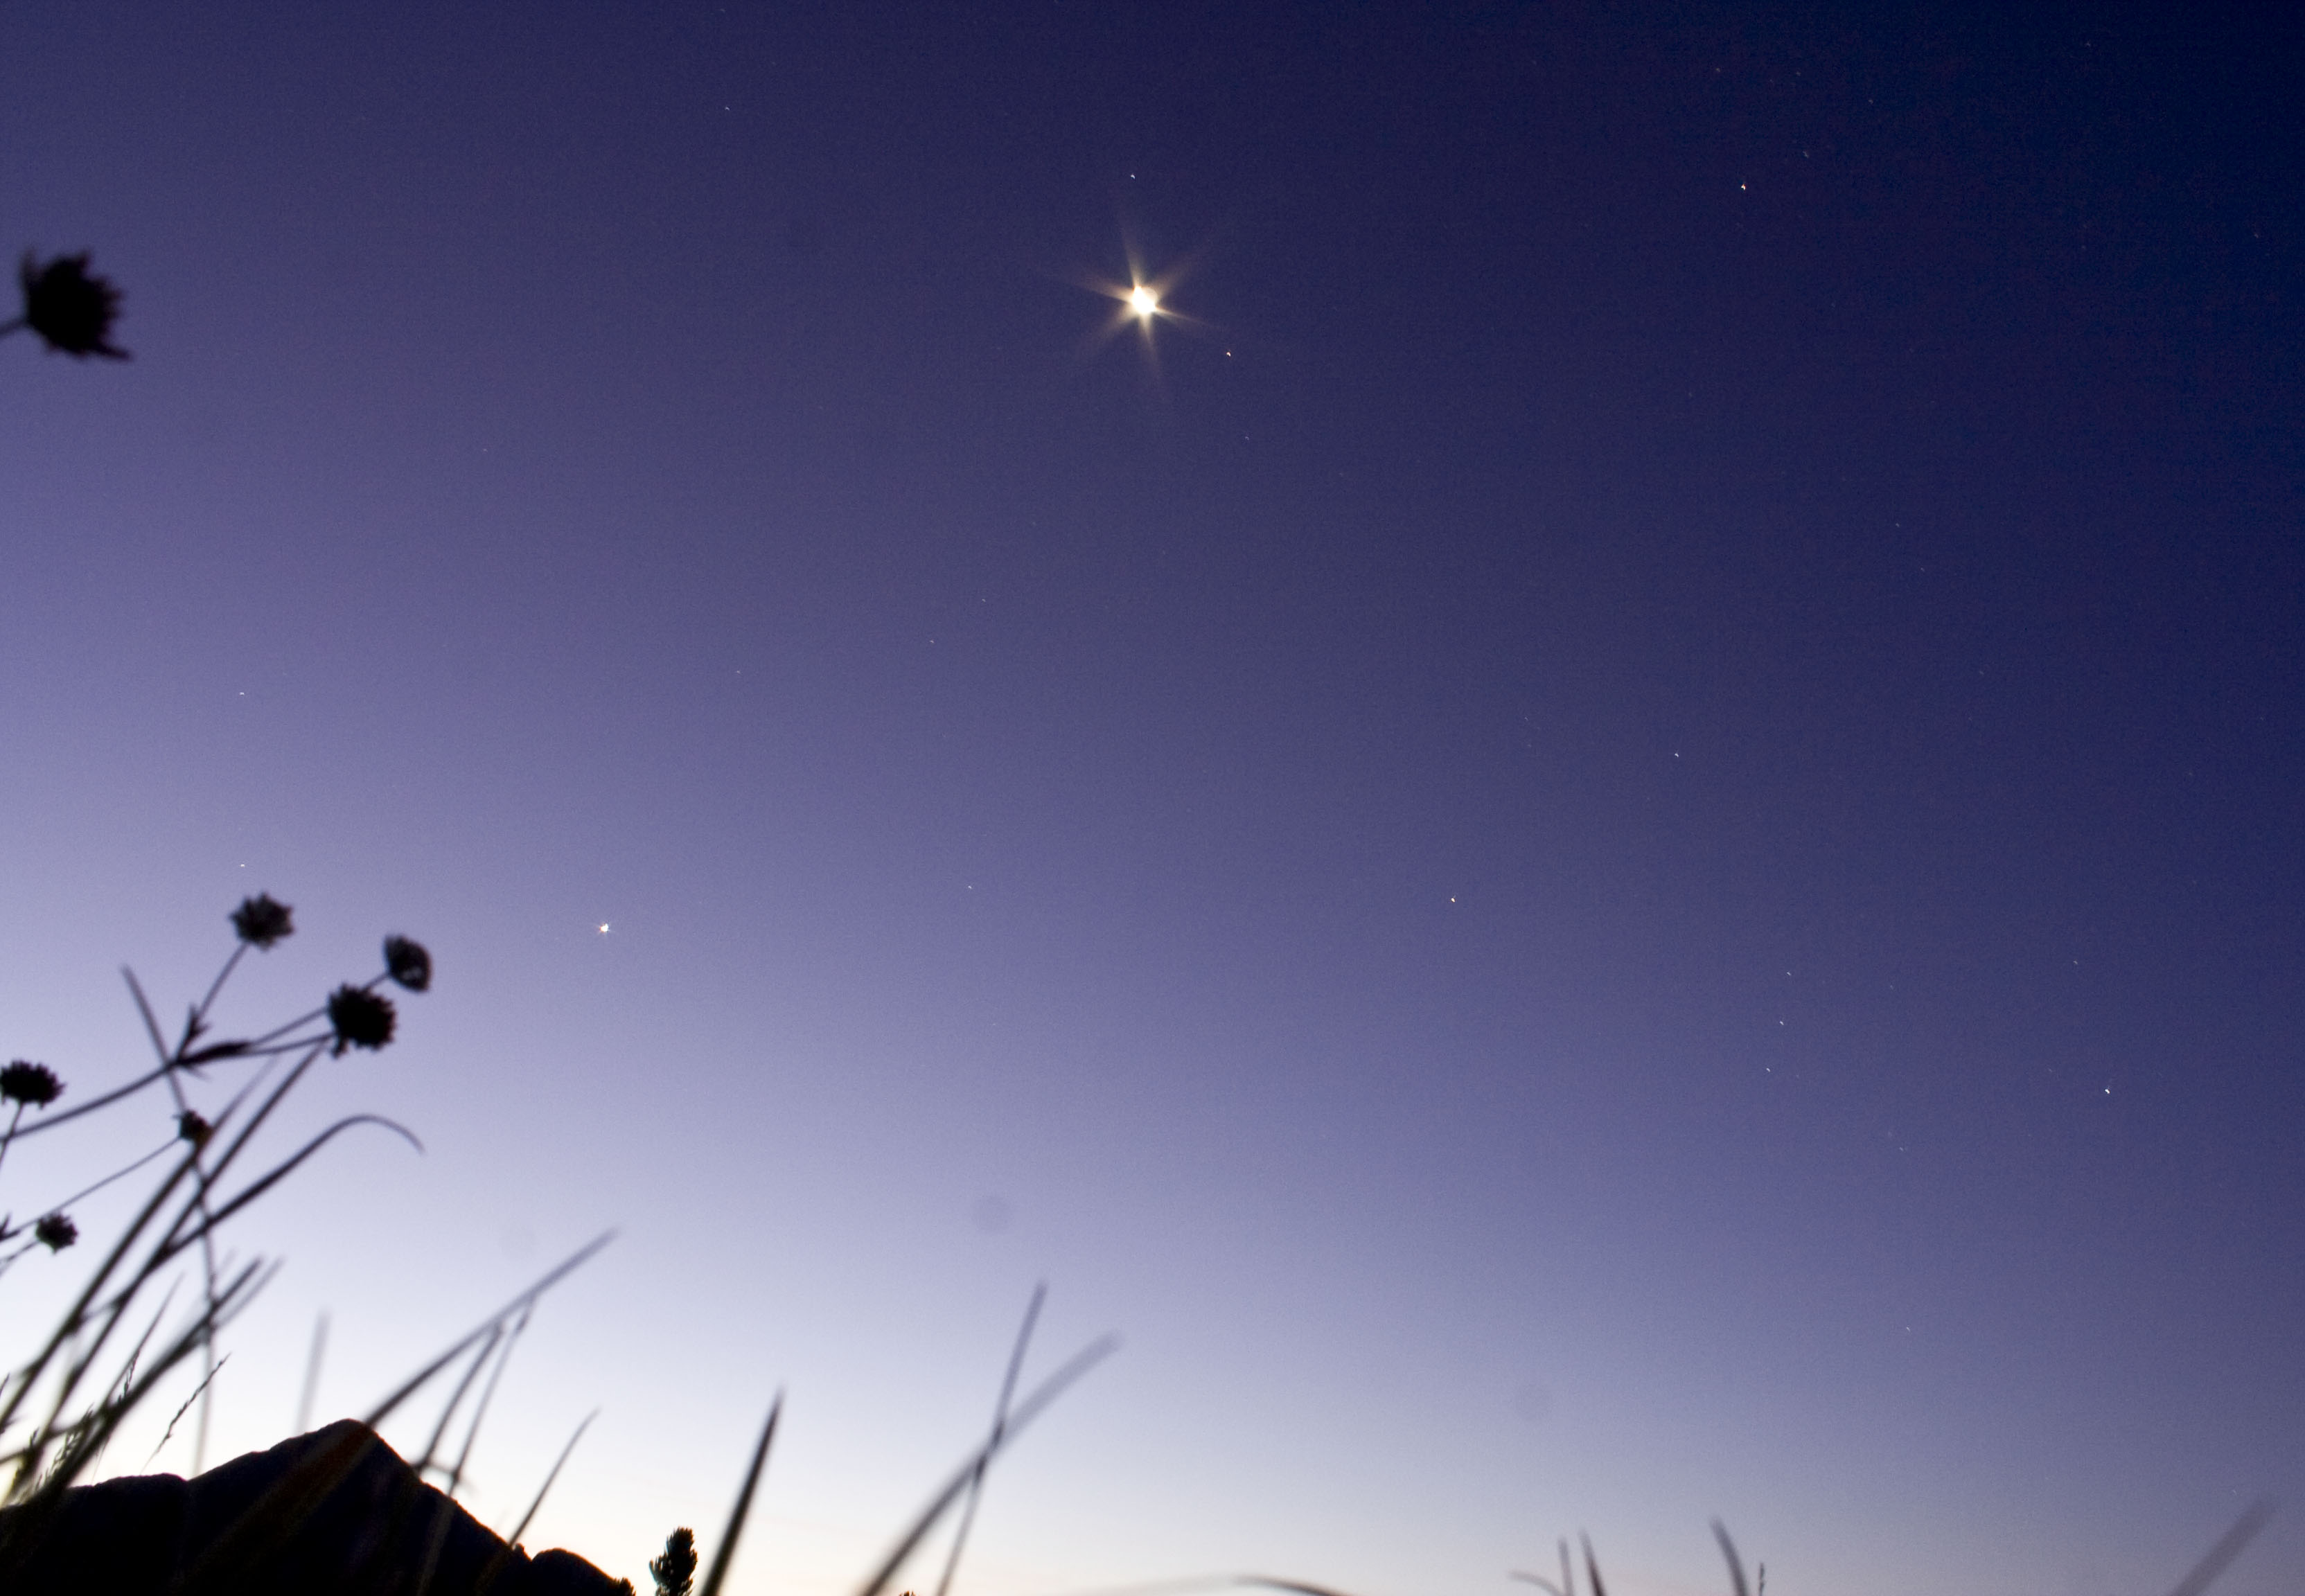
\includegraphics[width=\linewidth]{2009/m16-m12_through_trip/2009-Jana Carga - Canon 350d - 176_1--orig.jpg}} 
 \caption{Night on the \passage{Migovec plateau}. \pic{Jana Čarga}}
 \label{plataeu moon}
\end{marginfigure}


\recipecorner{Parathas}{All you need is:
\begin{itemize}
    \item 2 cups wholewheat flour
    \item Water
    \item Salt to taste
    \item 1 cup vegetable/ canola/ sunflower cooking oil (2 tbsps to knead the dough and the rest for frying the Parathas)
\end{itemize}
Mix it up, fry it like chapatis!
\mininame{Jarv}}



This year a few of us went up Mig; Đaljo, Špela, Erik, Tjaša and Karin.
As usual a stop at \passage{Kal} is necessary. Once on top, it was already dark
and most peoples were already asleep. The next day also Zec, Antonio
and Teja came up. We divided ourselves into three groups. Tetley did not
miss a chance to take Karin and Tjaša -- who were freshers on Mig -- caving
down \passage{M16} (\passage{Titanic}). In the end they ended up doing a
through trip and came out from \passage{M2}.


\begin{pagefigure}
\checkoddpage \ifoddpage \forcerectofloat \else \forceversofloat \fi
\frame{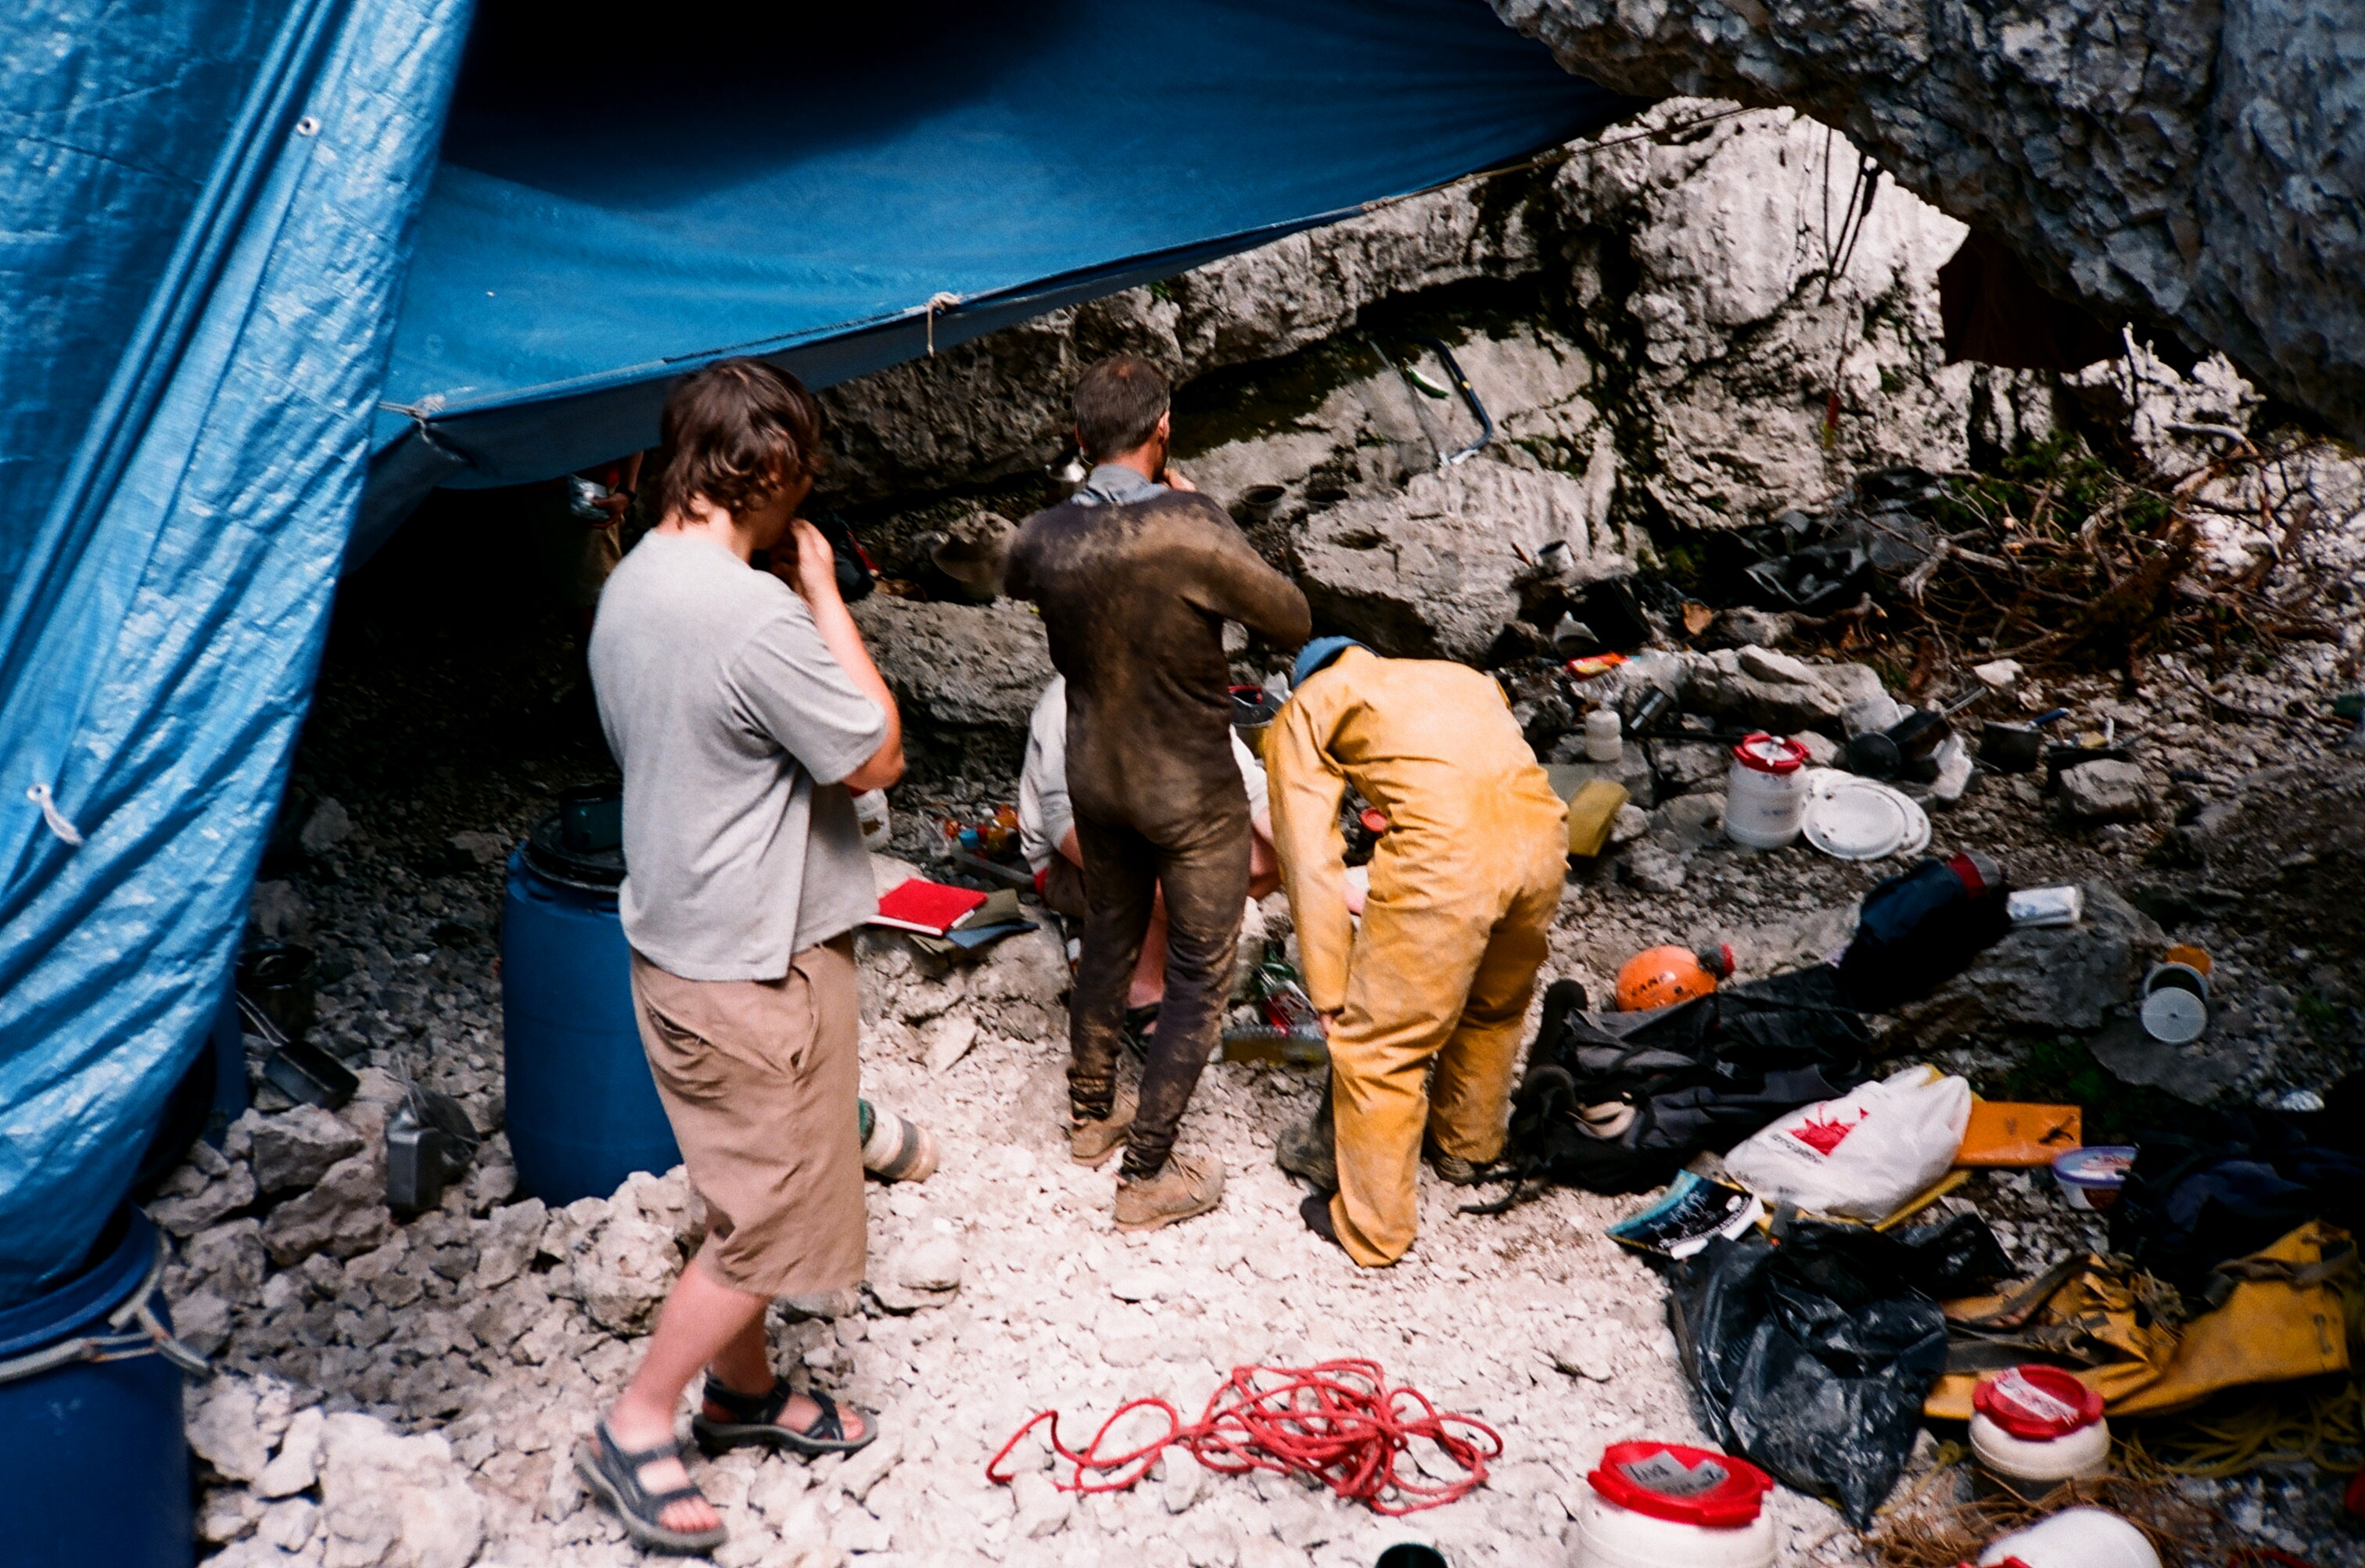
\includegraphics[width=\linewidth]{2009/m16-m12_through_trip/jarvist frost - olympus xa - superia 100 - tetley alex preparing in bivi--orig.jpg}}
\caption{Preparing for caving in the bivi. \pic{Jarvist Frost}}
\label{bivi cave prep}
\end{pagefigure}

I took Teja to the top of \passage{Pico} (\passage{Vrtnarija}) and back. The others went to
\passage{M16}.

We were all out in time for a traditional sunset gathering, which is
truly unforgivable.

The next day Tetley suggested doing the same through trip
(\passage{M16}-\passage{M2}) and at the same time check out one pitch in \passage{NCB}.
We liked the plan. The leaders were Karin and Tjaša followed by myself,
Erik and Thara. We all knew the way till \passage{Titanic}, but none of us
was in \passage{NCB} gallery before. We saw 3 pitches but were unsure as to
which pitch we needed to check out. We went all the way till the end of
the gallery and on the way back decided to check out the middle pitch.
We bolted and Thara went down first to check it out. He came back up
quickly with the news that there is no way on.


\tweet{8:09PM Jul 27, 2009}{2nd day of carry, now conc on UG camp and cave equip. JKP/MF off to piston GW to rig and check ropes, midnight call out. Weather lovely, ...}

At this point we decided
best to carry on with our loop trip. We were at \passage{Silos} now and
Tjaša went first down. There is a big traverse connecting \passage{M16}
with \passage{Silos}. I somehow managed to get stuck on it. After 20 min of
struggling I managed to get free. After that \passage{M2} - there was quite
a lot of nasty meanders to go through. After 8 hours we were finally
out. Back in the \passage{Bivi} we were laughing [over] which pitch we should check
out\ldots{}

\name{Iztok Možir}



\fullwidthbox{Main (big red A4) logbook: 17-08-09}{
Neither of us had been further in the system than \passage{Hotline} so
there was a bit of stumbling around to reach \passage{NCB}. Got to see some
of the big cave system has, that I would not see in the UK. When we
reached what we thought was the west end of \passage{NCB} the only thing we
could find that was possibly an undescended pitch described were two
large holes further back that connected at the bottom. However, there
were two holes at the bottom of that, one was descended one was not.
While James froze I descended 20 m to find very little at all and we
decided to head out. The way up was slightly marred when I sent a large
bolder down where James had been standing moments before. Otherwise we
got out in good time and slop was still lukewarm. We were told
afterwards that \passage{NCB} had a different west , so it is unclear where
we went.

\name{??}}


\begin{figure}[b!]
\checkoddpage \ifoddpage \forcerectofloat \else \forceversofloat \fi
\frame{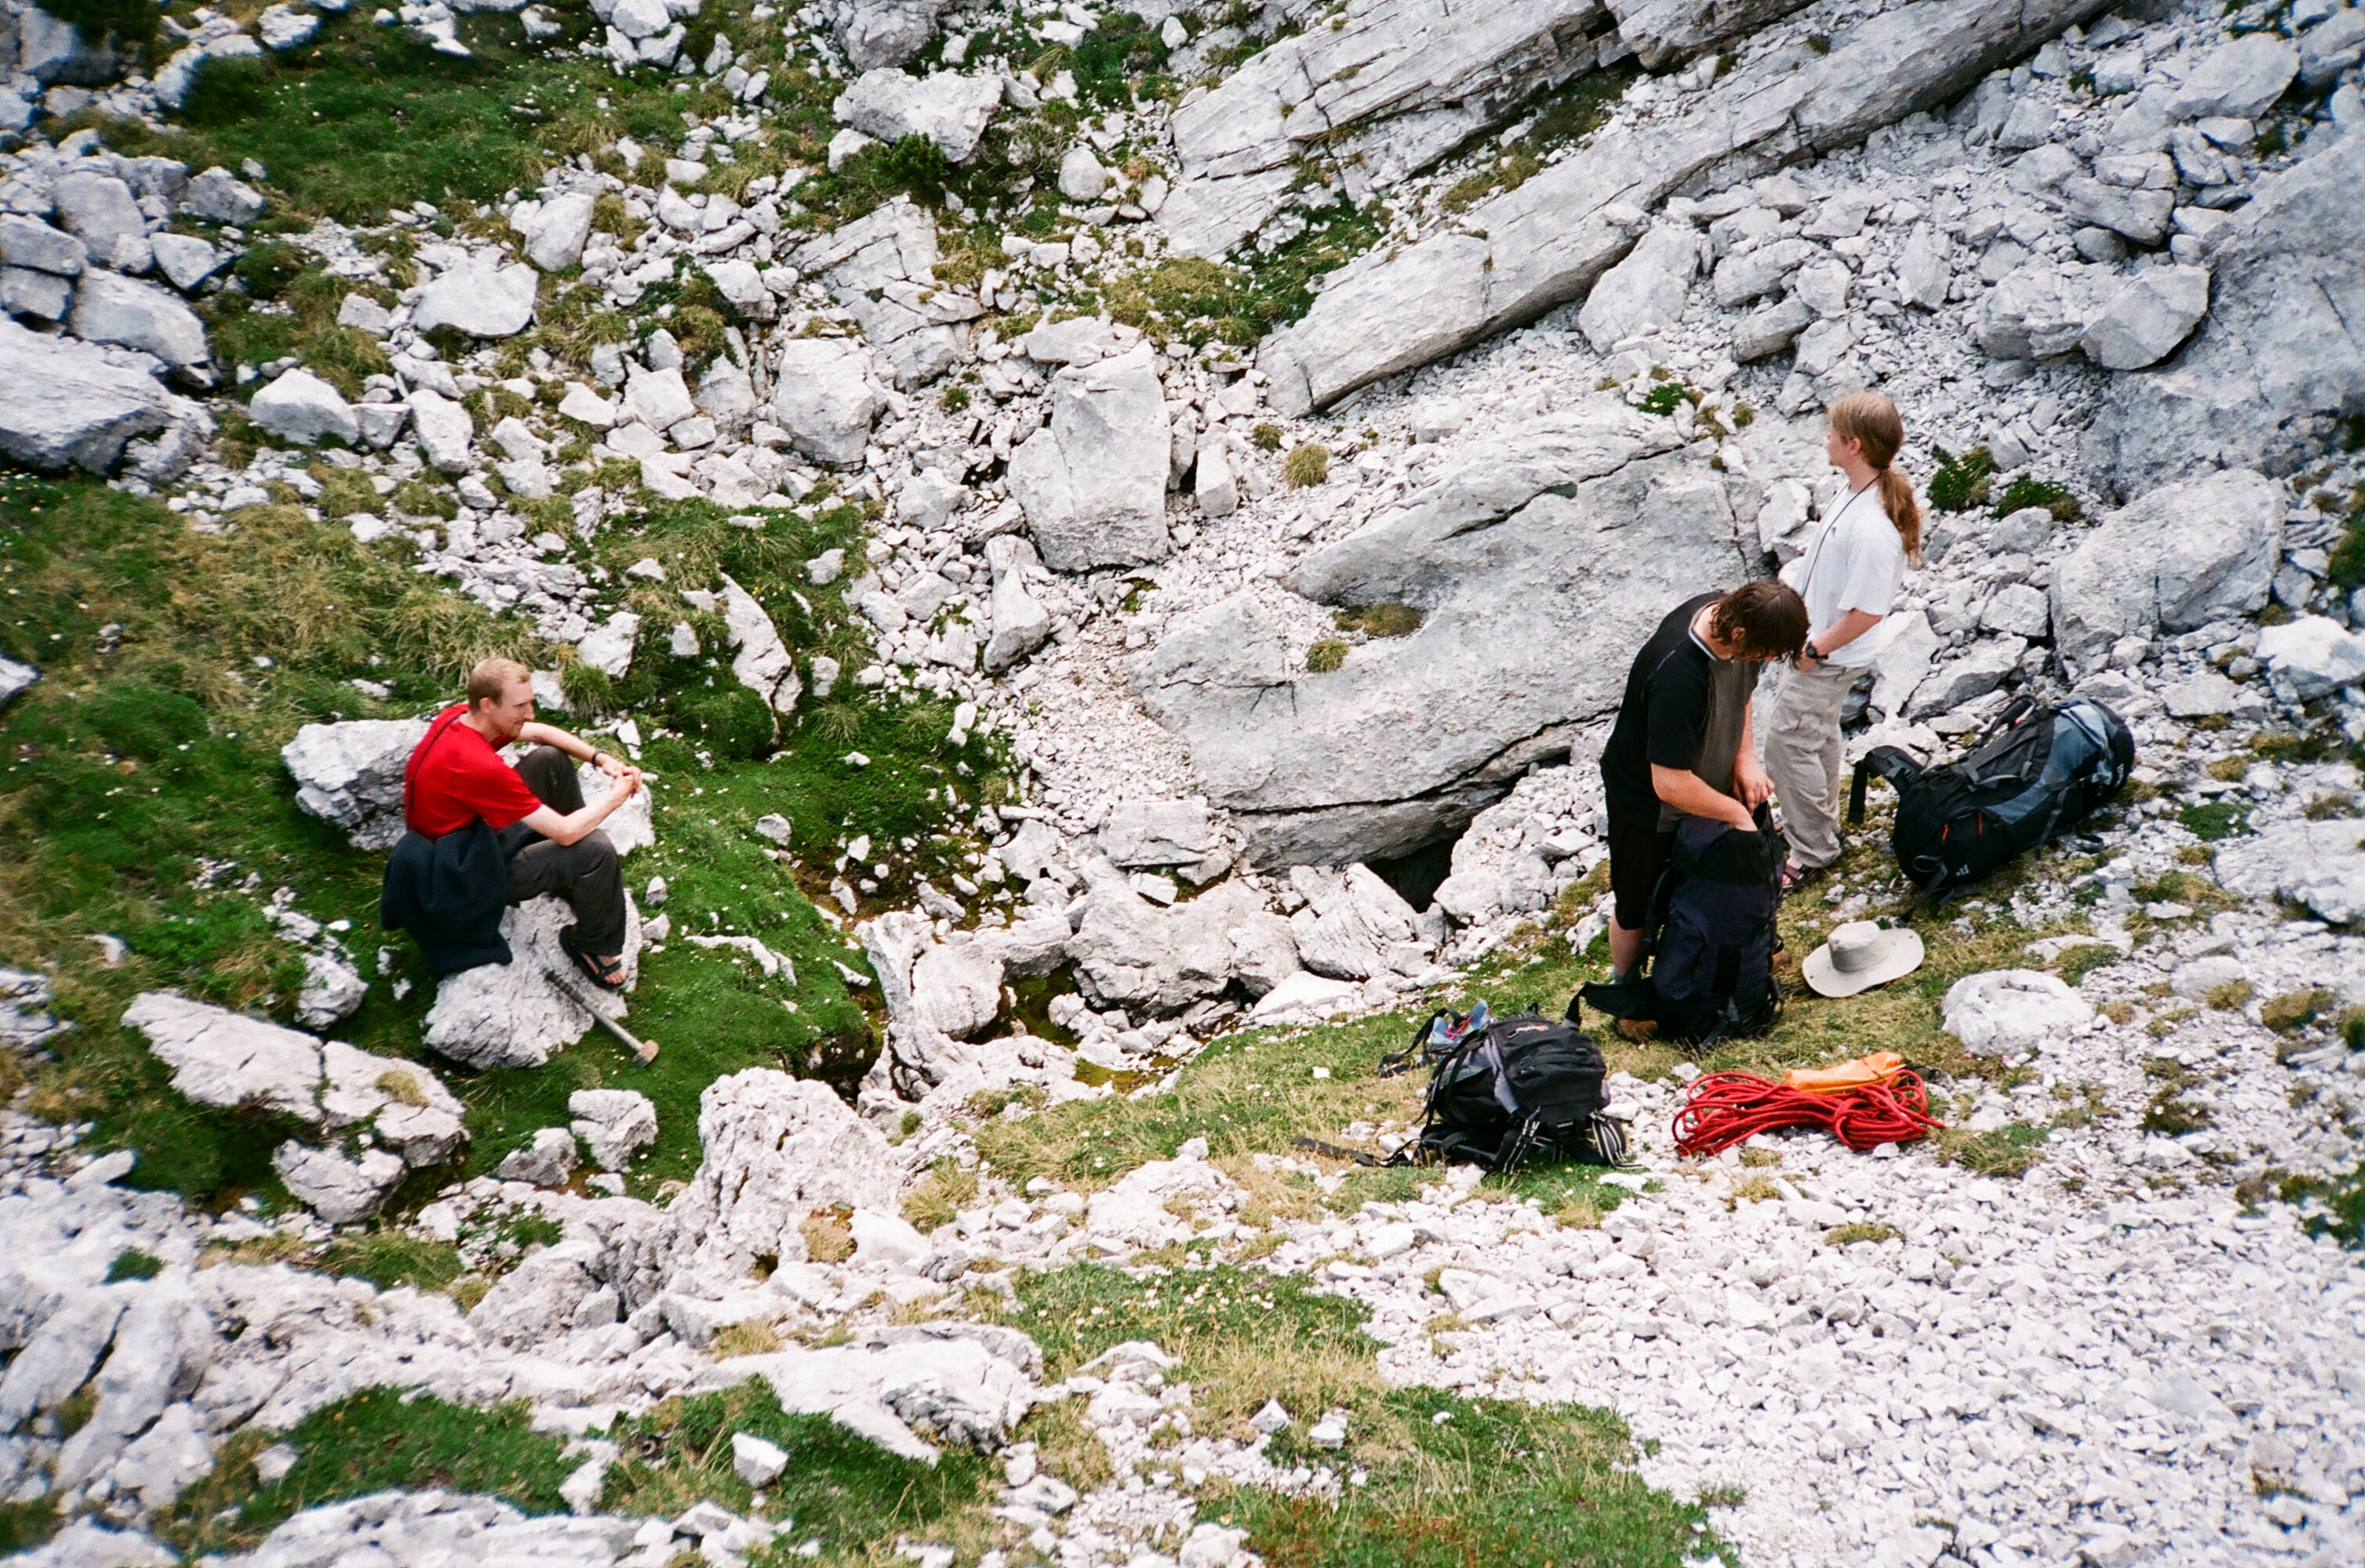
\includegraphics[width=\linewidth]{2009/collage/jarvist frost - olympus xa - superia 100 - william alex and andy at entrance to eastpole--orig.jpg}}
\caption{Andy Jurd, Alex Herriott and William French outside \protect\passage{Eastpole}, AKA \protect\passage{S1}. \pic{Jarvist Frost}}
\label{S1 eastpole 2009}
\end{figure}